\section{Elip}
\subsection{Tóm tắt lí thuyết}

\subsubsection{Định nghĩa}
Trong mặt phẳng cho hai điểm cố định $F_{1},F_{2}$ với $F_{1}F_{2}=2c$ và một độ dài không đổi $2a$ $(0<c<a)$.
\textit{Elip} $(E)$ là tập hợp tất cả các điểm $M$ trong mặt phẳng thỏa mãn $MF_{1}+MF_{2}=2a$.\\*
Ta gọi: 
\begin{itemize}
	\item $F_{1},F_{2}$ là các tiêu điểm của elip; 
	\item $F_{1}F_{2}=2c$: Tiêu cự của elip; 
	\item $MF_{1},MF_{2}$: Bán kính qua tiêu.
\end{itemize}
\begin{center}
	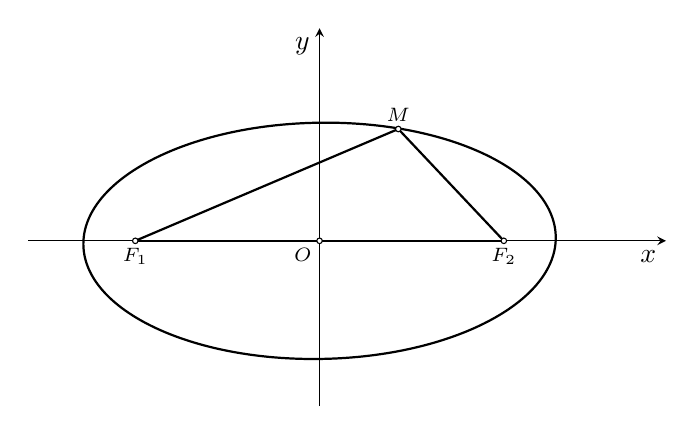
\begin{tikzpicture}[x=1.0cm,y=1.0cm,scale=1]
	\draw [rotate around={0.99:(0,0)},thick] (0,00) ellipse (3cm and 1.5cm);
	\draw [thick] (-2.34,0)-- (2.34,0);
	\draw [-stealth,thin] (-3.7,0) -- (4.4,0)node[below left] {$x$};
	\draw [-stealth,thin] (0,-2.1) -- (0,2.7)node[below left] {$y$};
	\draw [thick] (1,1.42)-- (-2.34,0);
	\draw [thick] (1,1.42)-- (2.34,0);
	\begin{scriptsize}
	\draw [fill=white] (-2.34,0) circle (1pt);
	\draw[color=black] (-2.34,0) node[below] {$F_1$};
	\draw [fill=white] (2.34,0) circle (1pt);
	\draw[color=black] (2.34,0) node[below] {$F_2$};
	\draw [fill=white] (1,1.42) circle (1pt);
	\draw[color=black] (1,1.42) node[above] {$M$};
	\draw [fill=white] (0,0) circle (1pt);
	\draw[color=black] (0,0) node[below left] {$O$};
	\end{scriptsize}
	\end{tikzpicture}
\end{center}
\subsubsection{Phương trình chính tắc của Elip}
Phương trình chính tắc của elip: $$\dfrac{x^{2}}{a^2}+\dfrac{y^{2}}{b^2}=1,$$
trong đó $a^2=b^2+c^2$.

\textbf{Chứng minh.}
Cho Elip có hai tiêu điểm $F_{1}$ và $F_{2}$. Chọn hệ trục tọa độ $Oxy$ sao cho $F_{1}(-c;0), F_{2}(c;0)$.\\*
Khi đó
$MF_{1}=\sqrt{(x+c)^{2}+y^{2}}\Leftrightarrow MF_{1}^{2}=(x+c)^{2}+y^{2}$\\*
$MF_{2}=\sqrt{(x-c)^{2}+y^{2}}\Leftrightarrow MF_{2}^{2}=(x-c)^{2}+y^{2}$\\*
$\Rightarrow MF_{1}^{2}-MF_{2}^{2}=4cx$ mà $M\in (E) \Leftrightarrow MF_{1}+MF_{2}=2a$ nên $MF_{1}-MF_{2}=\dfrac{2cx}{a}$.\\*
Ta có hệ
\begin{align}
\begin{cases}
MF_{1}-MF_{2} &=\dfrac{2cx}{a}\\
MF_{1}+MF_{2} &=2a \\
\end{cases}
\end{align}
Suy ra 
\begin{align}
\begin{cases}
MF_{1} &=a+\dfrac{cx}{a}\\&\\
MF_{2} &=a-\dfrac{cx}{a} \\
\end{cases}
\end{align}
Lại có: $MF_{1}=a+\dfrac{cx}{a}=\sqrt{(x+c)^{2}+y^{2}}$ hay $\left(a+\dfrac{cx}{a}\right)^{2}=(x+c)^{2}+y^{2}$\\*
Từ đó, phân tích và rút gọn ta được: $\dfrac{x^{2}}{a^2}+\dfrac{y^{2}}{a^{2}-c^{2}}=1$\\*
Do $a^{2}-c^{2}>0$ nên đặt $a^{2}-c^{2}=b^{2} \,(b>0)$, ta được:  $\boxed{\dfrac{x^{2}}{a^{2}}+\dfrac{y^{2}}{b^{2}}=1
	(*)}$\\*
Phương trình $(*)$ gọi là phương trình chính tắc của elip.
\subsubsection{Hình dạng của elip}
\begin{center}
	% Đồ thị hàm y=ax+b. Nếu hệ số lớn cần điều chỉnh hệ trục, vùng lưới, domain và lệnh \clip
	\begin{tikzpicture}[>=stealth,x=1cm,y=1cm,scale=2]
	\draw[->] (-2.25,0) -- (2.5,0) node[below] {\scriptsize $x$};
	\draw[->] (0,-1.25) -- (0,1.5) node[left] {\scriptsize $y$};
	\clip (-2.5,-1.5)rectangle(3,2);
\coordinate[label=below left:\scriptsize$O$] (O) at (0,0);
\draw (O) ellipse (2cm and 1cm); 
	\draw (-2,0)node[below left] {\scriptsize $A_1$}|-(0,1)node[above left] {\scriptsize $B_2$}-|(2,0)node[below right] {\scriptsize $A_2$}|-(0,-1)node[below left] {\scriptsize $B_1$}-| (-2,0)
	(-2,-1)node[below left] {\scriptsize $S$} (-2,1)node[above left] {\scriptsize $P$} (2,1)node[above right] {\scriptsize $Q$} (2,-1)node[below right] {\scriptsize $R$}
	;
	\coordinate [label=below left:\scriptsize$M$](M) at ($(0,0)+(60:2cm and 1cm)$); 
	\coordinate [label=below :\scriptsize$F_1$](F1) at (-1.7,0); 
	\coordinate [label=below :\scriptsize$F_2$](F2) at (1.7,0);
	\draw (F1)--(M)--(F2)
	;
	\end{tikzpicture}
	
	
\end{center}
\begin{enumerate}
	\item \textit{Trục đối xứng của elip}: 
	Elip có phương trình $(*)$ nhận các trục tọa độ làm trục đối xứng và nhận gốc tọa độ làm tâm đối xứng. 
	\item \textit{Hình chữ nhật cơ sở}:
	Vẽ qua ${A_1}$ và ${A_2}$ hai đường thẳng song song với trục tung, vẽ qua ${B_1}$ và ${B_2}$ hai đường thẳng song song với trục hoành. Bốn đường thẳng đó tạo thành hình chữ nhật $PQRS$. Ta gọi hình chữ nhật đó là hình chữ nhật cơ sở của elip.\\*
	Từ đó suy ra
	Mọi điểm của elip nếu không phải là đỉnh đều nằm trong hình chữ nhật cơ sở của nó, bốn đỉnh của elip là trung điểm các cạnh của hình chữ nhật cơ sở.\\*
	\begin{note}
		Các điểm: $A_{1}(-a;0);A_{2}(a;0);B_{1}(0;-b);B_{2}(0;b)$ gọi là các đỉnh của elip.\\*
		$A_{1}A_{2}=2a$: Độ dài trục lớn.
		$B_{1}B_{2}=2b$: Độ dài trục bé.\\*
	\end{note}
	\item \textit{Tâm sai của elip}:
	Tỉ số giữa tiêu cự và độ dài trục lớn của elip gọi là tâm sai của elip và được kí hiệu là $ e $ tức là $\boxed{e = \dfrac{c}{a}}$.\\*
	$ - $ Nếu tâm sai $ e $ càng bé (tức là càng gần $0$) thì b càng gần a và hình chữ nhật cơ sở càng gần với hình vuông, do đó đường elip càng “béo”.\\*
	$ - $ Nếu tâm sai $ e $ càng lớn (tức là càng gần $1$) thì tỉ số $\dfrac{b}{a}$ càng gần $1$ và hình chữ nhật cơ sở càng “dẹt”, do đó đường elip càng “gầy”.
\end{enumerate}

\subsection{Các dạng toán thường gặp}
\begin{dang}{Xác định các yếu tố của elip}
	Xác đinh tọa độ các đỉnh, tọa độ các tiêu điểm, độ dài các trục, độ dài tiêu cự của elip bằng cách áp dụng các công thức:
	\begin{enumerate}
		\item $c^2 = a^2 - b^2$.
		\item Độ dài trục lớn: $A_1 A_2 = 2a$, độ dài trục nhỏ: $B_1 B_2 = 2b$.
		\item Độ dài tiêu cự: $F_1 F_2 = 2c$.
	\end{enumerate}
\end{dang}
\begin{vd}%[0D3B1]
	Xác định tọa độ các đỉnh và độ dài các trục của các elip có phương trình sau:\\
	\begin{multicols}{2}
		\begin{enumerate}
			\item $\dfrac{x^2}{16}+\dfrac{y^2}{4}=1$;
			\item $x^2+4y^2=1$.
		\end{enumerate}
	\end{multicols}
	\loigiai{
		\begin{enumerate}
			\item 	Từ phương trình $\dfrac{x^2}{16}+\dfrac{y^2}{4}=1$, ta có $a=4$, $b=2$.\\
			Các đỉnh: $A_1(-4;0)$, $A_2(4;0)$, $B_1(0;-2)$, $B_2(0;2)$.\\
			Độ dài trục lớn: $A_1 A_2 = 2a = 8$, $B_1 B_2 = 2b = 4$.
			\\
			\item 	Ta có $x^2+4y^2=1 \Leftrightarrow \dfrac{x^2}{1}+\dfrac{y^2}{\frac{1}{4}}=1$ nên $a=1$, $b=\dfrac{1}{2}$.\\
			Các đỉnh $A_1(-1;0)$, $A_2(1;0)$, $B_1\left(0;-\dfrac{1}{2}\right)$, $B_2\left(0;\dfrac{1}{2}\right)$.\\
			Độ dài trục lớn: $A_1 A_2 = 2a = 2$, $B_1 B_2 = 2b = 1$.
		\end{enumerate}
	}
\end{vd}

\begin{vd}%[0D3B1]
	Xác định tọa độ các tiêu điểm và độ dài tiêu cự của các elip có phương trình sau:\\
	\begin{multicols}{2}
		\begin{enumerate}
			\item $\dfrac{x^2}{4}+\dfrac{y^2}{3}=1$
			\item $4x^2+25y^2=36$.
		\end{enumerate}
	\end{multicols}
	\loigiai{
		\begin{enumerate}
			\item Từ phương trình $\dfrac{x^2}{4}+\dfrac{y^2}{3}=1$, ta có $a^2=4$, $b^2=3$ nên $c=1$.\\
			Các tiêu điểm: $F_1(-1;0)$, $F_2(1;0)$.\\
			Độ dài tiêu cự: $F_1 F_2 = 2c = 2$.
			\item Ta có $4x^2+25y^2=36 \Leftrightarrow \dfrac{x^2}{9}+\dfrac{y^2}{\frac{36}{25}}=1$, suy ra: $a^2=9$, $b^2=\dfrac{36}{25} \Rightarrow c=\dfrac{3\sqrt{21}}{5}$.\\
			Các tiêu điểm $F_1\left(-\dfrac{3\sqrt{21}}{5};0\right)$, $F_2\left(\dfrac{3\sqrt{21}}{5};0\right)$.\\
			Độ dài tiêu cự: $F_1 F_2 = 2c = \dfrac{6\sqrt{21}}{5}$.
		\end{enumerate}
	}
\end{vd}

\begin{vd}%[0H3B3]
	Cho elip $(E)$ có độ dài trục lớn bằng $10$, tỉ số giữa tiêu cự và độ dài trục lớn là $\dfrac{3}{5}$. Tính độ dài trục nhỏ của elip.
	\loigiai{
		Ta có $2a=10 \Rightarrow a=5$. Mà $\dfrac{c}{a}=\dfrac{3}{5} \Rightarrow c=3$.\\
		Do đó $b^2=a^2-c^2=16 \Rightarrow b=4$.
		Vậy độ dài tục nhỏ $2b=8$.
	}
\end{vd}


\begin{center}
	\textbf{BÀI TẬP TỰ LUYỆN}
\end{center}

\begin{bt}%[0H3B3]
	Xác định tọa độ các đỉnh và các tiêu điểm của các elip có phương trình sau:
	\begin{multicols}{2}
		\begin{enumerate}
			\item $\dfrac{x^2}{100} + \dfrac{y^2}{64} = 1$;
			\item  $\dfrac{x^2}{4} + y^2 = 1$.
		\end{enumerate}
	\end{multicols}
	\loigiai{
		\begin{enumerate}
			\item Ta có $a^2=100, b^2=64 \Rightarrow a=10, b=8, c=6$.\\
			Vậy $A_1(-10;0)$, $A_2(10;0)$, $B_1(0;-8)$, $B_2(0;8), F_1(-6;0), F_2(6;0)$.
			\item Ta có $a^2=4, b^2=1 \Rightarrow a=2, b=1, c=\sqrt{3}$.\\
			Vậy $A_1(-2;0)$, $A_2(2;0)$, $B_1(0;-1)$, $B_2(0;1), F_1(-\sqrt{3};0), F_2(\sqrt{3};0)$.
		\end{enumerate}
	}
\end{bt}


\begin{bt}%[0H3B3]
	Xác định tọa độ các đỉnh và các tiêu điểm của các elip có phương trình sau:
	\begin{multicols}{2}
		\begin{enumerate}
			\item $16x^2+25y^2=1$;
			\item  $0{,}25 x^2+9y^2=1$.
		\end{enumerate}
	\end{multicols}
	\loigiai{
		\begin{enumerate}
			\item Ta có $16x^2+25y^2=1 \Leftrightarrow \dfrac{x^2}{\frac{1}{16}} + \dfrac{y^2}{\frac{1}{25}} = 1$.\\
			Do đó $A_1\left(-\dfrac{1}{4};0\right)$, $A_2\left(\dfrac{1}{4};0\right)$, $B_1\left(0;-\dfrac{1}{5}\right)$, $B_2\left(0;\dfrac{1}{5}\right)$, $ F_1\left(-\dfrac{3}{20};0\right)$, $ F_2\left(\dfrac{3}{20};0\right)$.
			\item Ta có $0,25 x^2+9y^2=1 \Leftrightarrow \dfrac{x^2}{4} + \dfrac{y^2}{\frac{1}{9}} = 1$.\\
			Vậy $A_1\left(-\dfrac{1}{4};0\right)$, $A_2\left(\dfrac{1}{4};0\right)$, $B_1\left(0;-\dfrac{1}{5}\right)$, $B_2\left(0;\dfrac{1}{5}\right), F_1\left(-\dfrac{3}{20};0\right), F_2\left(\dfrac{3}{20};0\right)$.
		\end{enumerate}
	}
\end{bt}

\begin{bt}%[0H3B3]
	Tìm độ dài trục lớn, trục nhỏ và tiêu cự của các elip có phương trình sau:
	\begin{multicols}{2}
		\begin{enumerate}
			\item $16x^2+64y^2=100$;
			\item  $\dfrac{x^2}{8} + \dfrac{y^2}{2} = 2$.
		\end{enumerate}
	\end{multicols}
	\loigiai{
		\begin{enumerate}
			\item Ta có $16x^2+64y^2=100 \Leftrightarrow \dfrac{x^2}{\frac{100}{16}} + \dfrac{y^2}{\frac{100}{64}} = 1$.
			Vậy $2a=5, 2b=\dfrac{5}{2}, 2c=\dfrac{5\sqrt{3}}{2}$.
			\item Ta có $\dfrac{x^2}{8} + \dfrac{y^2}{2} = 2 \Leftrightarrow \dfrac{x^2}{16} + \dfrac{y^2}{4} = 1$.
			Vậy $2a=8$, $2b=4$, $2c=4\sqrt{3}$.
		\end{enumerate}
	}
\end{bt}

\begin{bt}%[0H3B3]
	Xác định độ dài các trục của elip $(E)$: $\dfrac{x^2}{a^2} + \dfrac{y^2}{b^2} = 1$, $(a>b>0)$ biết rằng $(E)$ có độ dài tiêu cự bằng $6$ và đi qua điểm $A(5;0)$.
	\loigiai{
		Ta có $2c=6 \Rightarrow c=3$, $a=5 \Rightarrow b=4$.
		Vậy $2a=10$, $2b=8$.
	}
\end{bt}

\begin{bt}%[0H3K3]
	Xác định tọa độ các đỉnh của elip $(E)$: $\dfrac{x^2}{a^2} + \dfrac{y^2}{b^2} = 1$, $(a>b>0)$ biết rằng $(E)$ đi qua hai điểm $M(0;-2)$ và $N(2;\sqrt{3})$.
	\loigiai{
		Ta có $b=2$. $(E)$ đi qua điểm $N(2;\sqrt{3})$ nên $a^2=16 \Rightarrow a=4$.\\
		Vậy $A_1(-4;0)$, $A_2(4;0)$, $B_1(0;-2)$, $B_2(0;2)$.
	}
\end{bt}

\begin{bt}%[0H3K3]
	Cho elip $(E)$: $\dfrac{x^2}{a^2} + \dfrac{y^2}{b^2} = 1$. Biết $(E)$ đi qua điểm $M\left(2\sqrt{3};\dfrac{\sqrt{7}}{2}\right)$ và có tiêu cự bằng $\dfrac{3}{4}$ độ dài trục lớn. Tính độ dài trục nhỏ của $(E)$.
	\loigiai{
		Ta có $c=\dfrac{3}{4}a$, $b^2=a^2-c^2=\dfrac{7}{16}a^2$. Vì $M\in (E)$ nên $b^2=7$. Suy ra $2b=2\sqrt{7}$.
	}
\end{bt}


\begin{bt}%[0H3G3]
	Tìm tọa độ các đỉnh của elip $(E)$ có phương trình chính tắc là $\dfrac{x^2}{a^2} + \dfrac{y^2}{b^2} = 1$, biết rằng $(E)$ đi qua điểm $M(2;1)$ và các đỉnh trên trục nhỏ nhìn hai tiêu điểm dưới một góc vuông.
	\loigiai{
		Gọi $B$ là đỉnh trên trục nhỏ, $F_1$, $F_2$ là hai tiêu điểm. \\
		Khi đó tam giác $F_1BF_2$ vuông cân nên $b=c$. Do đó $a^2=b^2+c^2=2b^2$.\\
		Mặt khác $M\in (E)$ nên $\dfrac{4}{a^2} + \dfrac{1}{b^2} = 1$. Từ đó suy ra $b^2=3$, $a^2=6$.\\
		Vậy $A_1(-\sqrt{6},0)$, $A_2(\sqrt{6},0)$, $B_1(0; -\sqrt{3})$, $B_2(0;\sqrt{3})$.
	}
\end{bt}

\begin{bt}%[0H3G3]
	Cho elip $(E)$ có phương trình chính tắc là $\dfrac{x^2}{a^2} + \dfrac{y^2}{b^2} = 1$. Xác định tọa độ các tiêu điểm của $(E)$ biết rằng $(E)$ đi qua điểm $M(\sqrt{5};1)$ và khoảng cách từ một đỉnh nằm trên trục lớn đến một đỉnh nằm trên trục nhỏ bằng tiêu cự.
	\loigiai{
		Gọi $A(a;0)$, $B(0;b)$ là hai đỉnh.
		Khi đó $AB=2c$ suy ra $a^2+b^2=4c^2$.\\
		Mà $c^2=a^2-b^2$ nên $3a^2=5b^2$.\\
		Vì $M\in (E)$ suy ra $b^2=4$, $a^2=\dfrac{20}{3} \Rightarrow c=\dfrac{2\sqrt{6}}{3}$.\\
		Vậy $F_1\left(-\dfrac{2\sqrt{6}}{3};0\right)$, $F_1\left(-\dfrac{2\sqrt{6}}{3};0\right)$.
	}
\end{bt}

\begin{dang}{Viết phương trình chính tắc của elip}
Viết phương trình elip là quá trình tìm các yếu tố đặc trưng của elip bao gồm độ dài trục lớn ($2a$) và độ dài trục nhỏ ($2b$).
\begin{enumerate}[Bước 1.]
	\item Giả sử phương trình elip có dạng $(E)\colon\dfrac{x^{2}}{a^{2}}+\dfrac{y^{2}}{b^{2}}=1$.
	\item Từ những giả thiết bài toán, giải tìm $a$, $b$ và viết phương trình. 
\end{enumerate}
\begin{note}
	Khi làm bài cần chú ý các tính chất sau của elip:
	\begin{enumerate}
		\item Elip nhận hai trục $Ox,Oy$ làm trục đối xứng. 
		\item Tâm sai của elip $e=\dfrac{c}{a}$.
		\item Bán kính qua tiêu của điểm $M(x;y)\in (E)$: $MF_1=a+ex; MF_2=a-ex$.
		\item Đường chuẩn của elip:\\Đường thẳng $d_1: x+\dfrac{a}{e}=0$ được gọi là đường chuẩn của elip, ứng với tiêu điểm $F_1(-c;0)$.\\Đường thẳng $d_2: x-\dfrac{a}{e}=0$ được gọi là đường chuẩn của elip, ứng với tiêu điểm $F_2(c;0).$      
	\end{enumerate}
\end{note}
\end{dang}
\begin{vd}%[0H3Y5]
	Lập phương trình chính tắc của elip $(E)$ mà độ dài trục lớn bằng  $6$, độ dài trục nhỏ bằng $4$.
	\loigiai{Giả sử phương trình elip có dạng $(E)\colon \dfrac{x^{2}}{a^{2}}+\dfrac{y^{2}}{b^{2}}=1$.\\Độ đài trục lớn bằng $6\Rightarrow 2a=6\Rightarrow a=3$.\\Độ dài trục nhỏ bằng $4\Rightarrow 2b=4\Rightarrow b=2.$\\Vậy phương trình elip là $\dfrac{x^{2}}{9}+\dfrac{y^{2}}{4}=1$.  }   
\end{vd}
\begin{vd}%[0H3Y5]
	Lập phương trình chính tắc của elip $(E)$ có độ dài trục lớn bằng $10$, tiêu cự có độ dài bằng $6$.
	\loigiai{Giả sử phương trình elip có dạng $(E)\colon \dfrac{x^{2}}{a^{2}}+\dfrac{y^{2}}{b^{2}}=1$.\\
		Độ dài trục lớn bằng $10\Rightarrow 2a=10\Rightarrow a=5.$\\
		Độ dài tiêu cự bằng $6\Rightarrow 2c=6\Rightarrow c=3.$\\
		Ta có $b^{2}=a^{2}-c^{2}\Rightarrow b=4$.\\
		Vậy phương trình elip có dạng $\dfrac{x^{2}}{25}+\dfrac{y^{2}}{16}=1.$    }   
\end{vd}
\begin{vd}%[0H3Y5]
	Viết phương trình chính tắc của elip đi qua hai điểm $M(1;0), N\left(\dfrac{\sqrt{3}}{2};1\right).$
	\loigiai{Giả sử phương trình elip có dạng $(E)\colon \dfrac{x^{2}}{a^{2}}+\dfrac{y^{2}}{b^{2}}=1 $.\\
		Điểm $M\in (E)\Rightarrow \dfrac{1}{a^{2}}=1\Rightarrow a=1.$\\
		Điểm $N\in(E)\Rightarrow \dfrac{3}{4}+\dfrac{1}{b^{2}}=1\Rightarrow b=2.$\\
		Vậy phương trình chính tắc của elip có dạng $\dfrac{x^{2}}{1}+\dfrac{y^{2}}{4}=1 $.  } 
\end{vd}
\begin{center}
	\textbf{BÀI TẬP TỰ LUYỆN }
\end{center}
\begin{bt}%[0H3K5]
	Lập phương trình chính tắc của elip biết elip đi qua điểm $M(8;12)$ và có bán kính qua tiêu điểm bên phải của $M$ bằng $20$.
	\loigiai{Giả sử phương trình elip có dạng $(E)\colon \dfrac{x^{2}}{a^{2}}+\dfrac{y^{2}}{b^{2}}=1 $.\\
		$M(8;12)\in (E)\Rightarrow \dfrac{64}{a^{2}}+\dfrac{144}{b^{2}}=1.\\$ 
		Bán kính qua tiêu điểm bên phải $$ MF_2=20\Rightarrow a-ex=20\Rightarrow a-\dfrac{8c}{a}=20\Rightarrow c=\dfrac{a^{2}-20a}{8}.$$
		Lại có $b^{2}=a^{2}-c^{2}$, thay vào ta được phương trình ẩn $a$ sau khi quy đồng và khử mẫu có dạng
		\begin{eqnarray*}
			&&a^{4}-40a^{3}+272a^{2}+2560a-12288=0\\
			&\Leftrightarrow&(a-4)(a-16)(a^{2}-20a-192)=0\\
			&\Rightarrow&\hoac{a&=4\\a&=16\\a&=10-2\sqrt{73}\\a&=10+2\sqrt{73}.}
		\end{eqnarray*} 
		Chú ý là $c>0\Rightarrow a=10+2\sqrt{73}\Rightarrow c=24\Rightarrow b^{2}=40\sqrt{73}-184$.\\
		Vậy phương trình elip cần tìm là: $\dfrac{x^{2}}{(10+2\sqrt{73})^{2}}+\dfrac{y^{2}}{40\sqrt{73}-184}=1.$      
	}     
\end{bt}
\begin{bt}%[0H3K5]
	Viết phương trình chính tắc của elip đi qua $M\left(\dfrac{8}{\sqrt{5}};\dfrac{4}{\sqrt{5}}\right)$ và $\widehat{F_1MF_2}=90^{\circ}$.
	\loigiai{Giả sử phương trình elip có dạng $(E)\colon \dfrac{x^{2}}{a^{2}}+\dfrac{y^{2}}{b^{2}}=1 $.\\
		$M\in (E)\Rightarrow \dfrac{64}{5a^{2}}+\dfrac{16}{5b^{2}}=1(1)$.\\
		Ta có: $\vec{F_1M}=\left(\dfrac{8}{\sqrt{5}}+c;\dfrac{4}{\sqrt{5}}\right)$; $ \vec{F_2M}=\left(\dfrac{8}{\sqrt{5}}-c;\dfrac{4}{\sqrt{5}}\right)$ nên
		$\vec{F_1M}.\vec{F_2M}=0\Rightarrow c=4.$\\
		Lại có $b^{2}=a^{2}-c^{2}$. Thay vào $(1)$, ta có phương trình ẩn $a$: $\dfrac{64}{5a^{2}}+\dfrac{16}{5(a^{2}-16)}=1$ .\\
		Giải phương trình trên ta có $\hoac{a^{2}=\dfrac{80+16\sqrt{5}}{5}\\a^{2}=\dfrac{80-16\sqrt{5}}{5}.}$\\ Với $a>c\Rightarrow a^{2}=\dfrac{80+16\sqrt{5}}{5}$;
		$b^{2}=a^{2}-c^{2}=\dfrac{16\sqrt{5}}{5}$.\\
		Vậy phương trình elip cần tìm là: $\dfrac{x^{2}}{\dfrac{80+16\sqrt{5}}{5}}+\dfrac{y^{2}}{\dfrac{16\sqrt{5}}{5}}=1.$     
	} 
\end{bt}
\begin{bt}%[0H3K5]
	Viết phương trình chính tắc của đường elip biết hình chữ nhật cơ sở của $(E)$ có một cạnh nằm trên đường thẳng $y-2=0$ và có độ dài đường chéo bằng $6.$
	\loigiai{Giả sử phương trình elip có dạng $(E)\colon \dfrac{x^{2}}{a^{2}}+\dfrac{y^{2}}{b^{2}}=1 $.\\
		Một cạnh của hình chữ nhật cơ sở nằm trên đường thẳng $y=2$ suy ra $ b=2.$\\
		Đường chéo của hình chữ nhật cơ sở có độ dài bằng $6$ suy ra  $4a^{2}=36-16=20\Rightarrow a^{2}=5.$\\
		Vậy phương trình elip cần tìm là $\dfrac{x^{2}}{5}+\dfrac{y^{2}}{4}=1.$ 
	}   
\end{bt}
\begin{bt}%[0H3K5]
	Trong mặt phẳng toạ độ $Oxy$, cho hình thoi $ABCD$ có $AC=2BD$ và đường tròn tiếp xúc với các cạnh của hình thoi có phương trình $x^{2}+y^{2}=4$. Viết phương trình chính tắc của  elip đi qua các đỉnh $A,B,C,D$ của hình thoi. Biết điểm $A$ nằm trên trục $Ox$.
	\loigiai{ \immini{
			Đường tròn nội tiếp hình thoi $ABCD$ có tâm trùng với giao điểm của hai đường chéo $AC,BD$ của hình thoi.\\
			Do $A\in Ox\Rightarrow C\in Ox, B,D\in Oy$. Nên $A,B,C,D$ chính là bốn đỉnh của $(E)$.  \\
			Giả sử phương trình elip có dạng $(E)\colon \dfrac{x^{2}}{a^{2}}+\dfrac{y^{2}}{b^{2}}=1 .$
			}{
			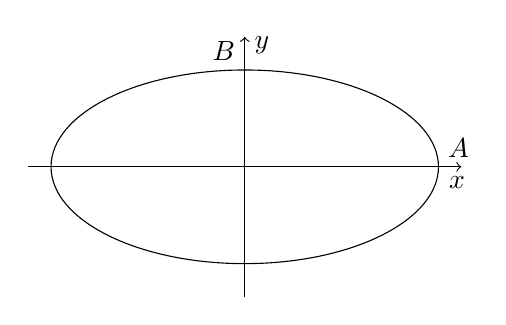
\begin{tikzpicture}[scale=0.55]
			\def\xmin{-5} \def\xmax{5}
			\def\ymin{-3} \def\ymax{3}
			\coordinate [label=60:$A$] (A) at (4.472,0);
			\coordinate [label=120:$B$] (B) at (0,2.237);
			\tkzDefPoints{0/0/O, 2/0/Z, 0/-2.237/D, -4.472/0/C}
			\tkzDrawCircle[radius](O,Z)
			\tkzDrawPoints(A,B,C,D)
			\tkzDrawSegments(A,B B,C C,D D,A)
			\tkzLabelPoints(D,O)
			\tkzLabelPoints[left](C)
			\draw[->](\xmin,0)--(\xmax,0); \draw(\xmax-0.1,0) node[below]{$x$};
			\draw[->](0,\ymin)--(0,\ymax); \draw(0,\ymax-0.2) node[right]{$y$};
			\draw (0,0) ellipse [x radius=4.473cm, y radius =2.236cm];
			\end{tikzpicture}}
		\noindent Từ việc bốn đỉnh của hình thoi là bốn đỉnh của hình thoi và giả thiết $AC=2BD$ suy ra $ a=2b$.\\
		Xét tam giác vuông $OAD$ trong hệ mặt phẳng $Oxy$ với $AD$ là tiếp tuyến của đường tròn nội tiếp hình thoi $ABCD$, đường  cao xuất phát từ đỉnh $O$ của tam giác này có độ dài là $h$ bằng bán kính đường tròn nội tiếp hình thoi $ABCD$.\\
	Ta có $\dfrac{1}{h^{2}}=\dfrac{1}{OA^{2}}+\dfrac{1}{OD^{2}}$, với $h=2, OA=a=2b=2OD$.\\
Từ đó ta có $a^{2}=20,b^{2}=5$.\\
Vậy phương trình elip cần tìm là $\dfrac{x^{2}}{20}+\dfrac{y^{2}}{5}=1.$
	}
\end{bt}
\begin{bt}%[0H3K5]
	Trong mặt phẳng với hệ toạ độ $Oxy$, cho điểm $M(1;2)$ và đường tròn \break$(C)\colon x^{2}+y^{2}=21$. Viết phương trình chính tắc của elip $(E)$ biết hình chứ nhật cơ sở của $(E)$ nội tiếp đường tròn $(C)$ và điểm $M$ nhìn hai tiêu điểm của $(E)$ dưới một góc $60^{\circ}$.  
	\loigiai{Giả sử phương trình elip có dạng $(E)\colon \dfrac{x^{2}}{a^{2}}+\dfrac{y^{2}}{b^{2}}=1 $.\\
		Vì đường tròn $(C)$ có tâm $O(0;0)$ trùng với tâm của hình chữ nhật cơ sở và tâm của elip nên ta có $2\sqrt{a^{2}+b^{2}}=2R$ suy ra $ a^{2}+b^{2}=21.$\\
		Ta có hai tiêu điểm $F_1(-c;0)$, $F_2(c;0)$, lại có $\widehat{F_1MF_2}=60^{\circ}$\\$\Rightarrow (F_1F_2)^{2}=(MF_1)^{2}+(MF_2)^{2}-2MF_1.MF_2.\cos60^{\circ}$\\
		$\Rightarrow 4c^{2}=(2+c)^{2}+1+(2-c)^{2}+1-\sqrt{1+(2+c)^{2}}.\sqrt{1+(2+c)^{2}}$\\
		$\Rightarrow 3c^{4}-34c^{2}+75=0\Leftrightarrow\hoac{&c^{2}=3\\&c^{2}=\dfrac{25}{3}.}$\\
		Với $c^{2}=3\Rightarrow a^{2}=12$, $b^{2}=9\Rightarrow (E)\colon \dfrac{x^{2}}{25}+\dfrac{y^{2}}{9}=1$.\\
		Với $c^{2}=\dfrac{25}{3}\Rightarrow a^{2}=\dfrac{44}{3}$, $b^{2}=\dfrac{19}{3}\Rightarrow (E)\colon \dfrac{x^{2}}{\frac{44}{3}}+\dfrac{y^{2}}{\frac{19}{3}}=1$.          
	}       
\end{bt}
\begin{bt}%[0H3K5]
	Trong mặt phẳng $Oxy$, cho đường tròn $(C)$ có phương trình $x^{2}+y^{2}=9$, viết phương trình chính tắc của cho elip $(E)$ có tâm sai $e=\dfrac{1}{3}$. Biết $(E)$ cắt $(C)$ tại $4$ điểm phân biệt $A,B,C,D$ sao cho $AB$ song song với $Ox$ và $AB=3BC.$
	\loigiai{Giả sử phương trình elip có dạng $(E)\colon \dfrac{x^{2}}{a^{2}}+\dfrac{y^{2}}{b^{2}}=1. $\\
		Tâm sai của $(E)$ bằng $\dfrac{1}{3}$ suy ra $ \dfrac{c}{a}=\dfrac{1}{3}\Rightarrow 8a^{2}-9b^{2}=0.\qquad (1)$\\
		Toạ độ của $A,B,C,D$ là nghiệm của hệ $\heva{x^{2}+y^{2}=9\qquad(2)\\\dfrac{x^{2}}{a^{2}}+\dfrac{y^{2}}{b^{2}}=1.\qquad(3)}$\\
		Do $(E)$ và $(C)$ cùng nhận $Ox,Oy$ làm trục đối xứng nên ta có $ABCD$ là hình chữ nhật.\\    
		Giả sử $A(x;y),$ vì $AB \parallel Ox$ nên $B(-x;y); C(-x;-y); D(x;-y).$\\
		Ta có $AB=3BC\Leftrightarrow x^{2}=9y^{2}.\qquad (4)$\\
		Từ $(2)$ thay vào $(4)$ ta có: $x^{2}=\dfrac{81}{10}, y^{2}=\dfrac{9}{10}$, thay vào $(3)$, ta được $\dfrac{81}{a^{2}}+\dfrac{9}{b^{2}}=1.\qquad (5)$\\
		Từ $(1)$ và $(5)$ ta có hệ sau $\heva{8a^{2}-9b^{2}=0\\\dfrac{81}{a^{2}}+\dfrac{9}{b^{2}}=1}$ $\Leftrightarrow\heva{a^{2}=\dfrac{729}{80}\\b^{2}=\dfrac{81}{10}.}$\\
		Vậy phương trình elip $(E)$ cần tìm là $\dfrac{x^{2}}{\frac{729}{80}}+\dfrac{y^{2}}{\frac{81}{10}}=1.$                   }         
\end{bt}

\Closesolutionfile{ans}